\documentclass[11pt]{amsart}
%prepared in AMSLaTeX, under LaTeX2e
\addtolength{\oddsidemargin}{-.5in} 
\addtolength{\evensidemargin}{-.5in}
\addtolength{\topmargin}{-.35in}
\addtolength{\textwidth}{1.2in}
\addtolength{\textheight}{0.7in}

\renewcommand{\baselinestretch}{1.08}

\usepackage{fancyvrb} % for "comment" environment

\newcommand{\mfile}[1]{
\begin{quote}
\bigskip
\VerbatimInput[frame=single,label=\fbox{\normalsize \textsl{\,#1\,}},fontfamily=courier,fontsize=\scriptsize]{#1}
\end{quote}
}

\usepackage{hyperref}
\usepackage{xspace}

\newtheorem*{thm}{Theorem}
\newtheorem*{defn}{Definition}
\newtheorem*{example}{Example}
\newtheorem*{problem}{Problem}
\newtheorem*{remark}{Remark}

\usepackage[final]{graphicx}


% macros
\usepackage{amssymb}
\newcommand{\bA}{\mathbf{A}}
\newcommand{\bB}{\mathbf{B}}
\newcommand{\bE}{\mathbf{E}}
\newcommand{\bF}{\mathbf{F}}
\newcommand{\bJ}{\mathbf{J}}
\newcommand{\br}{\mathbf{r}}
\newcommand{\bx}{\mathbf{x}}
\newcommand{\hbi}{\mathbf{\hat i}}
\newcommand{\hbj}{\mathbf{\hat j}}
\newcommand{\hbk}{\mathbf{\hat k}}
\newcommand{\hbn}{\mathbf{\hat n}}
\newcommand{\hbr}{\mathbf{\hat r}}
\newcommand{\hbt}{\mathbf{\hat t}}
\newcommand{\hbx}{\mathbf{\hat x}}
\newcommand{\hby}{\mathbf{\hat y}}
\newcommand{\hbz}{\mathbf{\hat z}}
\newcommand{\hbphi}{\mathbf{\hat \phi}}
\newcommand{\hbtheta}{\mathbf{\hat \theta}}
\newcommand{\complex}{\mathbb{C}}
\newcommand{\ppr}[1]{\frac{\partial #1}{\partial r}}
\newcommand{\ppt}[1]{\frac{\partial #1}{\partial t}}
\newcommand{\ppx}[1]{\frac{\partial #1}{\partial x}}
\newcommand{\ppy}[1]{\frac{\partial #1}{\partial y}}
\newcommand{\ppz}[1]{\frac{\partial #1}{\partial z}}
\newcommand{\pptheta}[1]{\frac{\partial #1}{\partial \theta}}
\newcommand{\ppphi}[1]{\frac{\partial #1}{\partial \phi}}
\newcommand{\Div}{\ensuremath{\nabla\cdot}}
\newcommand{\Curl}{\ensuremath{\nabla\times}}
\newcommand{\curl}[3]{\ensuremath{\begin{vmatrix} \hbi & \hbj & \hbk \\ \partial_x & \partial_y & \partial_z \\ #1 & #2 & #3 \end{vmatrix}}}
\newcommand{\cross}[6]{\ensuremath{\begin{vmatrix} \hbi & \hbj & \hbk \\ #1 & #2 & #3 \\ #4 & #5 & #6 \end{vmatrix}}}
\newcommand{\eps}{\epsilon}
\newcommand{\grad}{\nabla}
\newcommand{\image}{\operatorname{im}}
\newcommand{\integers}{\mathbb{Z}}
\newcommand{\ip}[2]{\ensuremath{\left<#1,#2\right>}}
\newcommand{\lam}{\lambda}
\newcommand{\lap}{\triangle}
\newcommand{\note}[1]{[\scriptsize #1 \normalsize]}
\newcommand{\MatIN}[1]{\mtt{>> #1}}
\newcommand{\onull}{\operatorname{null}}
\newcommand{\rank}{\operatorname{rank}}
\newcommand{\range}{\operatorname{range}}
\renewcommand{\P}{\mathcal{P}}
\newcommand{\real}{\mathbb{R}}
\newcommand{\trace}{\operatorname{tr}}

\renewcommand{\Re}{\operatorname{Re}}
\renewcommand{\Im}{\operatorname{Im}}
\newcommand{\Arg}{\operatorname{Arg}}

\newcommand{\pf}{\textsc{Proof}.\xspace}

\newcommand{\Matlab}{\textsc{Matlab}\xspace}
\newcommand{\Octave}{\textsc{Octave}\xspace}
\newcommand{\MO}{\textsc{Matlab/Octave}\xspace}

\newcommand{\ppart}[1]{\textbf{(#1)}\, }
\newcommand{\epart}[1]{\medskip\noindent\quad\textbf{(#1)}\, }
\newcommand{\prob}[1]{\medskip\noindent\textbf{#1.}\quad }



\begin{document}
\scriptsize \noindent Math 310 Numerical Analysis, Fall 2010 (Bueler) \hfill \today
\normalsize\bigskip
\thispagestyle{empty}

\Large
\centerline{\textbf{Solutions to Assignment \#3}}
\normalsize

\medskip

\prob{1} \ppart{a} The Vandermonde system of equations is
\begin{align*}
a_0 + a_1 + a_2 &= 1 \\
a_0 + 3.5 a_1 + (3.5)^2 a_2 &= 7 \\
a_0 + 4 a_1 + 4^2 a_2 &= 5
\end{align*}
Entered into \MO:
\small \begin{quote}\begin{Verbatim}
>> A = [1 1 1; 1 3.5 3.5^2; 1 4 4^2];
>> b = [1 7 5]';
>> v = A \ b
v =
   -8.8667
   12.0000
   -2.1333
>> format rat
>> v
v =
    -133/15
         12
     -32/15
\end{Verbatim}
\end{quote} \normalsize
Thus the polynomial is $P(x) = -\frac{133}{15} + 12 x - \frac{32}{15} x^2$.  \quad (\emph{The ``\emph{\texttt{format rat}}'' command shows the result as rational numbers.  This is merely a convenience, and not fundamental at all.})


\epart{b} In the Newton form we start with the unknown polynomial $P(x) = c_0 + c_1(x-1) + c_2(x-1)(x-3.5)$.  Then the system of equations looks like
$$\begin{array}{lcl}
c_0      &=& 1 \\
c_0 + 2.5 c_1    &=& 7 \\
c_0 + 3 c_1 + 1.5 c_2  &=& 5
\end{array}$$
Again in \MO:
\small \begin{quote}\begin{Verbatim}
>> M = [1 0 0; 1 2.5 0; 1 3 1.5];
>> b = [1 7 5]';  % same b
>> format rat
>> w = M \ b
w =
          1
       12/5
     -32/15
\end{Verbatim}
\end{quote} \normalsize
Thus the polynomial is $P(x) = 1 + \frac{12}{5}(x-1) - \frac{32}{15}(x-1)(x-3.5)$.

\epart{c} The Lagrange polynomials are, in turn:
\begin{align*}
\ell_1(x) &= \frac{(x-3.5)(x-4)}{(1-3.5)(1-4)} = \frac{1}{7.5} (x-3.5)(x-4), \\
\ell_2(x) &= \frac{(x-1)(x-4)}{(3.5-1)(3.5-4)} = - \frac{1}{1.25} (x-1)(x-4), \\
\ell_3(x) &= \frac{(x-1)(x-3.5)}{(4-1)(4-3.5)} = \frac{1}{1.5} (x-1)(x-3.5), \\
\end{align*}
so $P(x) = \frac{2}{15} (x-3.5)(x-4) - \frac{28}{5} (x-1)(x-4) + \frac{10}{3} (x-1)(x-3.5)$.

\epart{d} Tedious but straightforward calculations show that the answers to \textbf{(b)} and \textbf{(c)} are identical to that in \textbf{(a)}, once they are put in monomial (standard) polynomial form.

\prob{2}  I wrote the following code:

\mfile{randsevenpoly.m}

The result I get in one particular run is shown in figure 1, and at the command line:

\begin{figure}[ht]
\includegraphics[width=0.5\textwidth]{randsevenpoly}
\caption{A typical polynomial of degree 6 going through 7 random points in the plane.}
\end{figure}

\small \begin{quote}\begin{Verbatim}
>> randsevenpoly
result:
  P(x) = -1.011475 + 79.872031 x + -300.181011 x^2 + -50.216815 x^3 ...
            + 721.891339 x^4 + -159.569729 x^5 + -326.084835 x^6
\end{Verbatim}
\end{quote} \normalsize

Your answer will \emph{not} be the same.\footnote{In fact, because it generates random points \texttt{x,y}, my program above produces a new output every time you run it.  This can even be a disadvantage, because it is harder to test for correctness if you do not have repeatability.  To get repeatability, one simple way is to compute the random points \emph{once} and then hard-code those numbers into the m-file.}

Now, I did not ask you if finding this polynomial \emph{was a good idea}.  If you have seven data points, should you put a degree six polynomial through the data?  Generally, should high degree polynomials be put through data points?  The answer is, generally, that if the points are not the values of a \emph{smooth} and \emph{precisely-known} function then you should \emph{not} use high-degree polynomial interpolation.  The interpolating polynomial will generally not be similar to the function ``behind'' your data.  Instead, low degree polynomial \emph{regression}, for instance linear regression, is likely to be a good idea if the the points are imperfect data. 

\prob{3} \emph{The solution method for lower triangular systems is very natural: start at the first equation and get the unknowns in turn.}

\epart{a} I solved the system by hand: $x=3$, $y=0$, $z=2$.

\epart{b}  The solution is straightforward to write, as long as it is understood that you \emph{must use these equations in the order they are given}.  That is, as unknowns $x_j$ become known, they can be used in the next equation:
\begin{align*}
x_1 &= \frac{b_1}{a_{11}} \\
x_2 &= \frac{b_2 - a_{21} x_1}{a_{22}} \\
& \dots \\
x_j &= \frac{b_j - a_{j1} x_1 - a_{j2} x_2 - \dots - a_{j,j-1} x_{j-1}}{a_{jj}} \\
 & \dots \\
x_n &= \frac{b_n - a_{n1} x_1 - a_{n2} x_2 - \dots - a_{n,n-1} x_{n-1}}{a_{nn}}
\end{align*}
\noindent The condition for success of this method is that all the $a_{jj}$ must be nonzero.  In that case there is a unique solution.


\prob{4}  \ppart{a} \ppart{b} \ppart{c} I wrote the following code which does all three parts.  The result is in left side of figure 2.

\mfile{smoothpolyapprox.m}

\begin{figure}[ht]
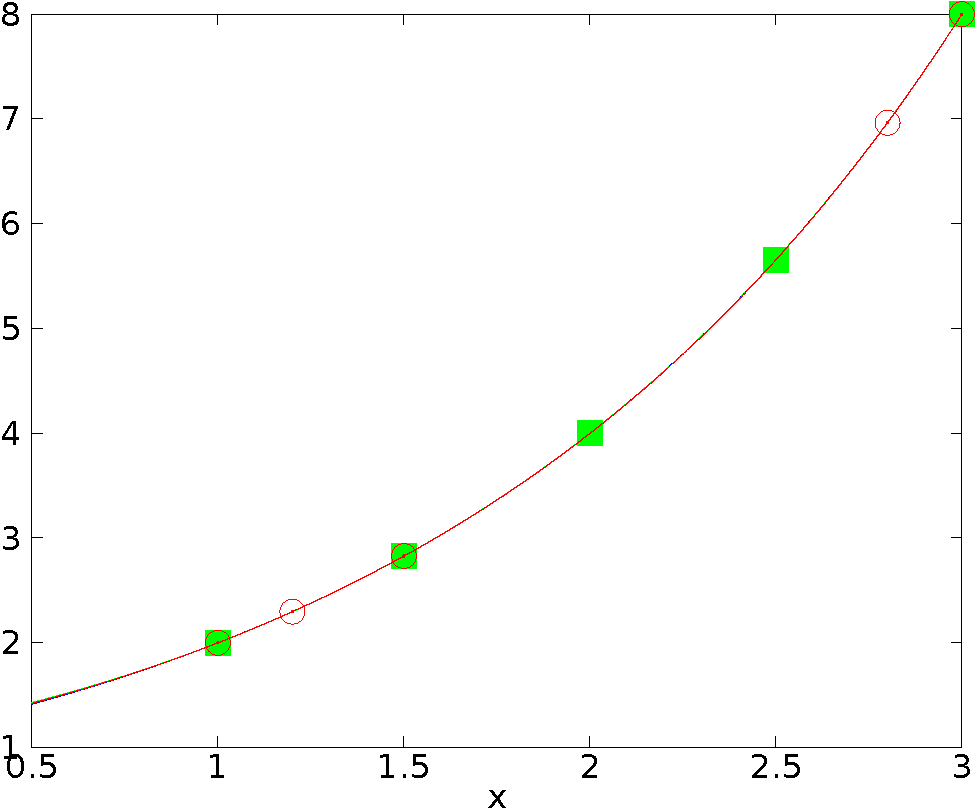
\includegraphics[width=0.45\textwidth]{smoothpolyapprox} \, 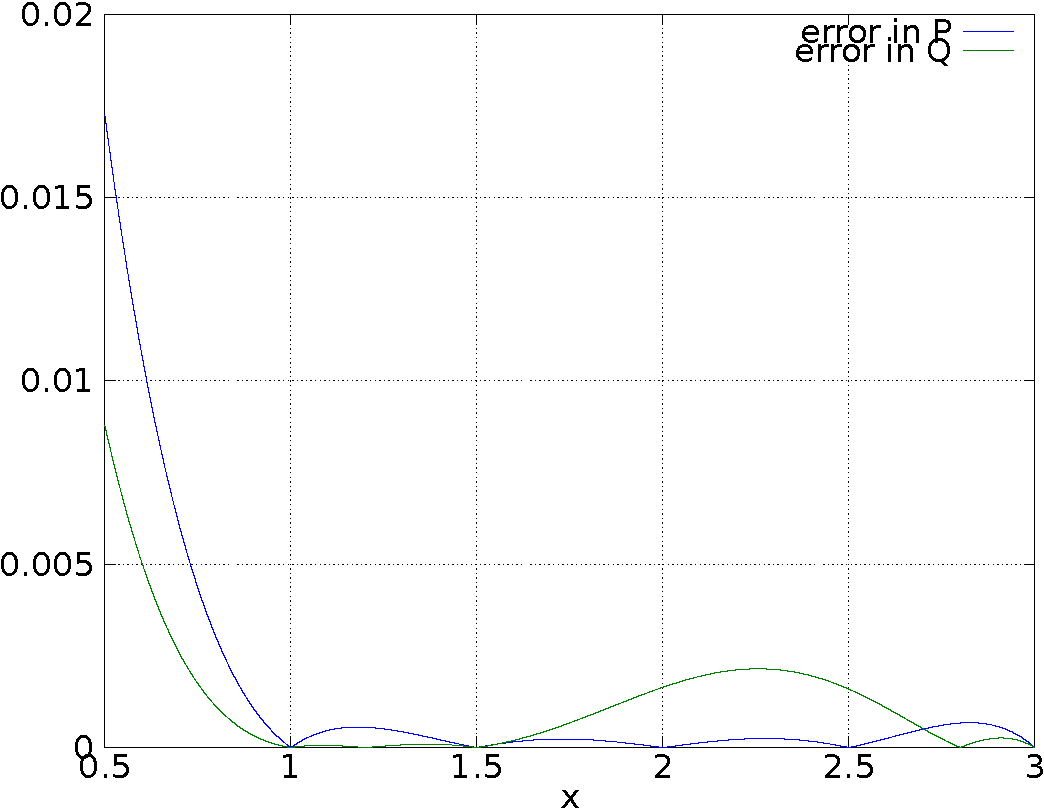
\includegraphics[width=0.45\textwidth]{clearpolyerror}
\caption{\textbf{(left)}  Degree 5 polynomials interpolating $y=2^x$ on the interval $[0.5,3]$ do an excellent job.  At screen resolution we cannot tell the difference between $y=2^x$, $y=P(x)$, and $y=Q(x)$.  The green squares show the interpolation points for $P$ and the red circles show the points for $Q$.  \textbf{(right)} Computing differences shows $P(x)$ is \emph{substantially} better than $Q(x)$.}
\end{figure}

The left part of Figure 2 raises the question: are these degree five polynomial interpolants equally good?  The answer is:  No, the error in $P(x)$ is more than four times smaller than in $Q(x)$.

You do not see that $P(x)$ is distinctly better than $Q(x)$ until you subtract:
\small\begin{quote}\begin{Verbatim}
>> figure, plot(xx,abs(2.^xx-P),xx,abs(2.^xx-Q)), grid on, xlabel x
>> legend('error in P','error in Q')
\end{Verbatim}
\end{quote}\normalsize
As shown in the right side of Figure 2, there is a much bigger error in $Q(x)$.  It has big errors in the ``big gap'' between $x_5=2$ and $x_6=3$ where $Q(x)$ uses no interpolation points.

\end{document}
